\documentclass[a4paper, 12pt]{article}

\usepackage{cmap}
\usepackage{mathtext} 
\usepackage[T2A]{fontenc}
\usepackage[utf8]{inputenc}
\usepackage[english,russian]{babel}	

\usepackage{amsfonts,amssymb,amsthm,mathtools}
\usepackage{amsmath}
\usepackage{icomma} 

\usepackage{graphicx} 
\graphicspath{{Picturies/}}
\usepackage{wrapfig}

\usepackage{array,tabularx,tabulary,booktabs}
\usepackage{longtable}
\usepackage{multirow}

\usepackage{caption}
\captionsetup{labelsep=period}

\renewcommand{\phi}{\varphi}
\newcommand{\eps}{\varepsilon}
\renewcommand{\AA}{\ensuremath{\mathring{A}}}
\newcommand{\parag}[1]{\paragraph*{#1:}}

\newcounter{Points}
\setcounter{Points}{1}
\newcommand{\point}{\arabic{Points}. \addtocounter{Points}{1}}

\author{Вязовцев Андрей, Б01-005}
\date{02.11.22}
\title{Лабораторная работа 5.4.1.}

\begin {document}

\maketitle

\parag {Цель работы} Измерить пробег $\alpha$-частиц в воздухе двумя способами и определить энергию частиц.

\parag {В работе используются} торцевой счётчик Гейгера, сцинтилляционный счётчик.

\parag {Теоретическая справка} ~\\

Явление радиоктивности состоит в самопроизвольном распаде ядер с испусканием одной или нескольких частиц. К числу радиоактивных процессов относятся $\alpha$- и $\beta$-распады (в том числе и $K$-захват), $\gamma$-излучение, деление ядер, а также испускание запаздывающих нейтронов и протонов. В нашей работе мы будем рассматривать первое явление.

При $\alpha$-распаде исходное родительское ядро испускает ядро гелия ($\alpha$-частицу) и превращается в дочернее ядро, число протонов и нейтронов которого меньше на две единицы. Функциональная связь между энергией $\alpha$-частицы $E$ и периодом полураспада радиоактивного ядра $T_{1/2}$ хорошо описывается формулой:

\begin{equation}
    lg T_{1/2} = \frac{a}{\sqrt{E}} + b
\end{equation}

Экспериментально энергию $\alpha$-частиц удобно определять по величине их пробега в веществе. Они, главным образом, теряют свою энегрию от неупругих столкновений с атомами вещества. Эти столкновения вызывают ионизацию и возбуждение атомов, поэтому такие потери называются ионизационными. 

В нашем рабочем диапазоне (от 4 до 9 МэВ) длину пробега можно вычислить с помощью следующей экспериментальной формулы:

\begin{equation}
    R = 0.32 E^{3/2}
    \label{eq:sc}
\end{equation}

где $R$ выражается в сантиметрах, а $E$ --- в МэВ.

\parag {Экспериментальная установка} ~

Энергию $\beta$-частиц определяют с помощью $\beta$-спектрометров. В работе используется магнитный спектрометр с <<короткой линзой>>. На рис. \ref{img:work1} изображена схема установки. А на рис. \ref{img:work2} --- общая блок-схема.

\begin{figure}[!h]
    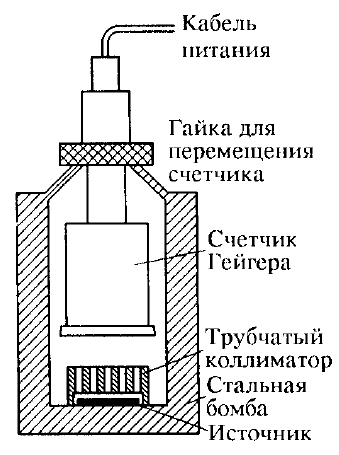
\includegraphics[scale = 0.4]{Workplace1}
    \centering
    \caption{Установка для измерения пробега $\alpha$-частиц с помощью торцевого счётчика Гейгера}
    \label{img:work1}
\end{figure}

\begin{figure}[!h]
    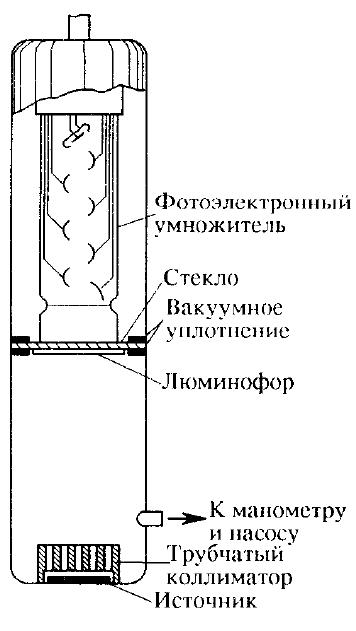
\includegraphics[scale = 0.4]{Workplace2}
    \centering
    \caption{Установка для измерения пробега $\alpha$-частиц с помощью сцинтилляционного счётчика}
    \label{img:work2}
\end{figure}

\begin{figure}[!h]
    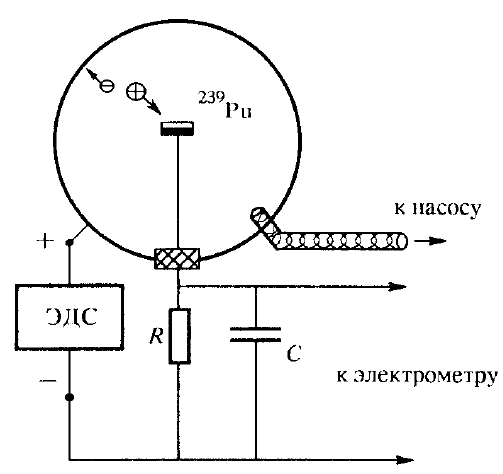
\includegraphics[scale = 0.4]{Workplace3}
    \centering
    \caption{Схема устройства ионизационной камеры}
    \label{img:work1}
\end{figure}

\parag {Ход работы} ~\\

\parag {I. Исследование пробега $\alpha$-частиц с помощью счётчика Гейгера} ~\\

\point Включим установку в сеть, дадим ей прогреться. Убедимся, что она <<чувствует>> $\alpha$-частицы. 

\point Снимем зависимость скорости счёта от расстояния $x$ от источника до приёмника. Результаты представлены в таблице \ref{tab:geig}.

\begin{table}[!h]
    \centering
    \begin{tabular}{|c|c|c|c|c|c|c|c|c|}
        \hline
        $t$, с & 70.218 & 40.162 & 40.212 & 44.857 & 76.341 & 125.074 & 120.178 & 40.209 \\ \hline
        $N$ & 907 & 657 & 603 & 612 & 506 & 42 & 26 & 581 \\ \hline
        $x$, мм & 10.0 & 12.0 & 14.0 & 16.0 & 18.0 & 20.0 & 25.0 & 15.0 \\ \hline
    \end{tabular}
    \\~\\
    \begin{tabular}{|c|c|c|c|c|c|c|c|c|}
        \hline
        $t$, с & 40.206 & 40.206 & 40.584 & 51.685 & 119.884 & 119.975 & 120.123 \\ \hline
        $N$ & 568 & 544 & 505 & 502 & 339 & 108 & 47 \\ \hline
        $x$, мм & 15.5 & 16.5 & 17.0 & 17.5 & 18.5 & 19.0 & 19.5 \\ \hline
    \end{tabular}
    \caption {Измерения на счётчике Гейгера}
    \label{tab:geig}
\end{table}

\point Построим график $\dfrac{N}{t} (x)$ и $\dfrac{d (N/t)}{dx} (x)$ (см. рис. \ref{img:geig}). Определим по нем средний и экстраполированный пробег $\alpha$-частиц.

Получаем: 

\begin{align*}
    R_{ср} &\approx 18 ~ мм \\
    R_э &= 19.2 \pm 1.2 ~ мм
\end{align*}

Т.~к. $p_{атм} = 99.6$ кПа, т.~е. плотность воздуха $\rho \approx 1.184 \cdot 10^{-3}~\dfrac{г}{см^3}$, то можно перевести величины в $\dfrac{г}{см^2}$:

\begin{align*}
    R_{ср} &\approx 2.1 \cdot 10^{-3} ~ \dfrac{г}{см^2} \\
    R_э &= (2.27 \pm 0.14) ~ \cdot 10^{-3} ~ \dfrac{г}{см^2}
\end{align*}

\begin{figure}[!h]
    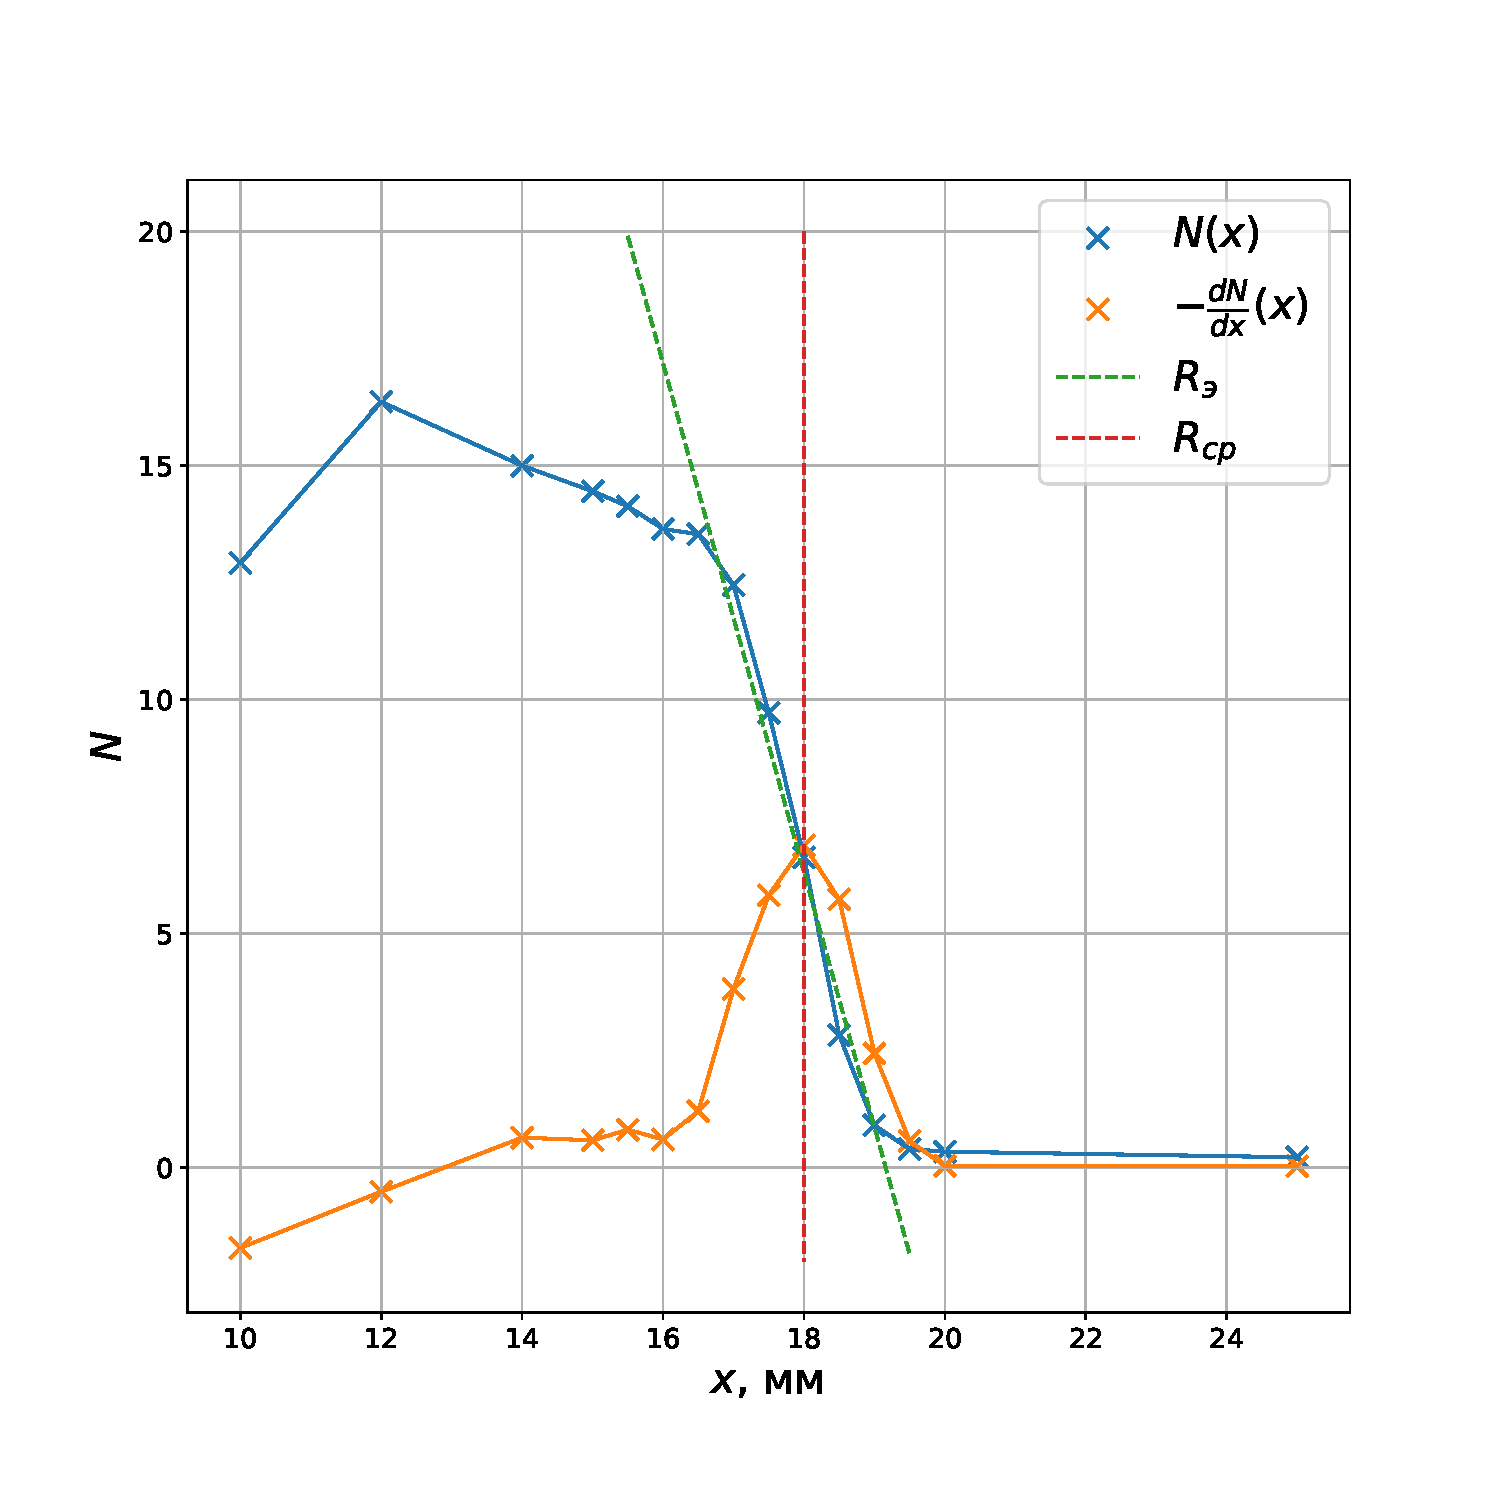
\includegraphics[scale = 0.4]{geig}
    \centering
    \caption{Красивый график $N(x)$}
    \label{img:geig}
\end{figure}

\newpage

\parag {II. Определение пробега $\alpha$-частиц с помощью сцинтилляционного счётчика} ~\\

\point Включим установку в сеть, дадим ей прогреться. Настроим её по инструкции.

\point Снимем зависимость $N (p)$. Результаты на таблице \ref{tab:sc}.

\begin{table}[!h]
    \centering
    \begin{tabular}{|c|c|c|c|c|c|c|c|c|}
        \hline
        $\Delta p$, мм.~рт.~ст. & 735 & 725 & 700 & 675 & 650 & 625 & 600 & 575 \\ \hline
        $N$ & 3582 & 3308 & 2932 & 2524 & 2123 & 3187 & 2125 & 2185 \\ \hline
        $t$, с & 10 & 10 & 10 & 10 & 10 & 20 & 20 & 40 \\ \hline
    \end{tabular}
    \\~\\
    \begin{tabular}{|c|c|c|c|c|c|c|c|}
        \hline
        $\Delta p$, мм.~рт.~ст. & 550 & 500 & 450 & 400 & 350 & 475 & 525 \\ \hline
        $N$ & 1677 & 489 & 80 & 15 & 7 & 342 & 723 \\ \hline
        $t$, с & 50 & 50 & 50 & 50 & 20 & 50 & 50 \\ \hline
    \end{tabular}
    \caption {Измерения на сцинтилляционном счётчике}
    \label{tab:sc}
\end{table}

\point Построим график $N (p)$, где $p = p_{атм} - \Delta p$, $p_{атм} = 747$~мм.~рт.~ст. Найдём, аналогично предыдущему пункту, $p_{ср}$ и $p_э$. Получаем:

\begin{align*}
    p_{ср} &\approx 147 ~ мм.~рт.~ст.  \\
    p_э &= (230 \pm 50) ~ мм.~рт.~ст.
\end{align*}

\begin{figure}[!h]
    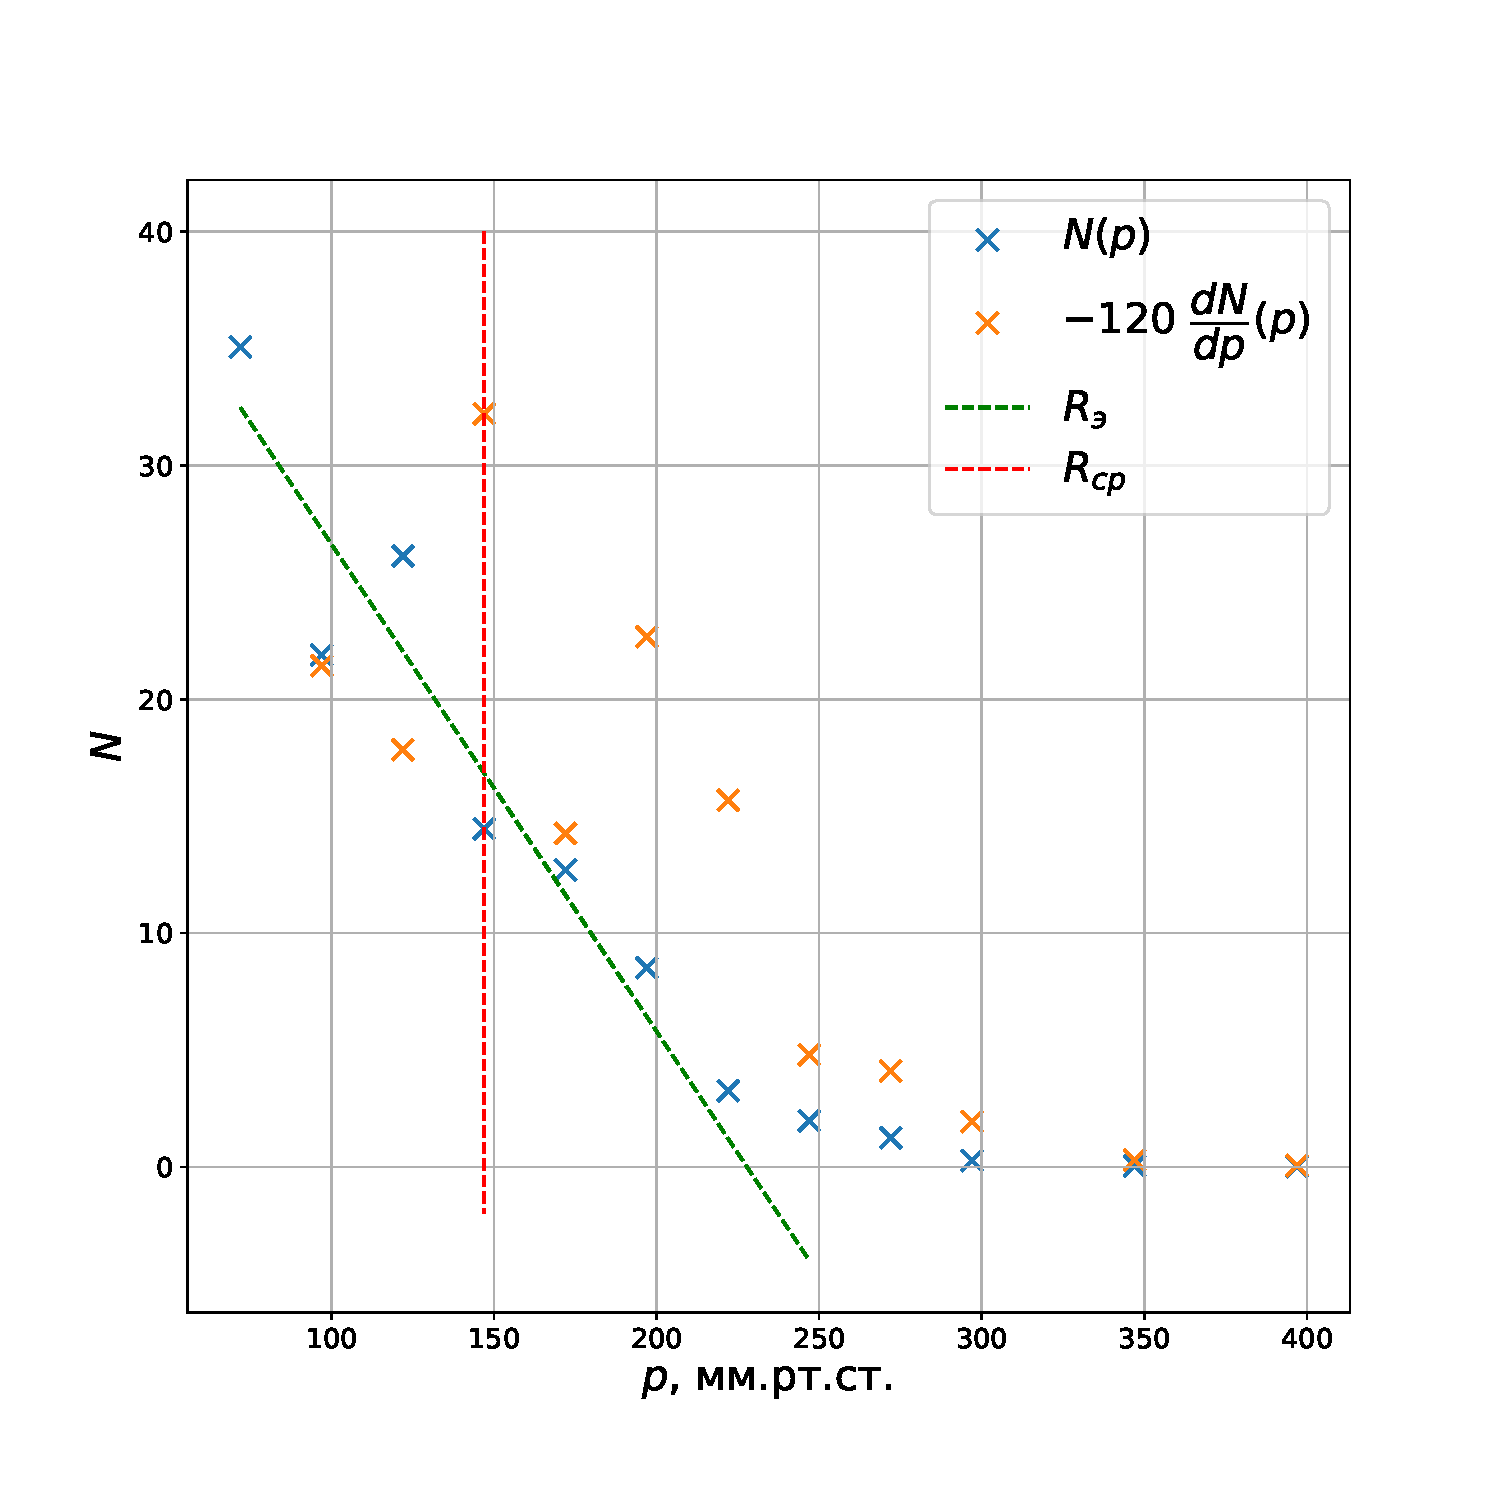
\includegraphics[scale = 0.4]{sc}
    \centering
    \caption{Красивый график $N(p)$}
    \label{img:sc}
\end{figure}

\point Пересчитаем пробег к $R$ при $p = 760$~мм.~рт.~ст. и $T = 288$ К. Учтём, что общая длина установки $9$ см.

% Ну и дерьмо редкостое получилось. И да, продублирую: 
% Интересно, для кого я пишу это в шесть часов ночи? Напиши, если реально читаешь это.

\begin{align*}
    R_{ср} &\approx 17 ~ мм = 2 \cdot 10^{-3} ~ \dfrac{г}{см^2} \\
    R_э &= (27 \pm 6) ~ мм = (3.2 \pm 0.7) \cdot 10^{-3} ~ \dfrac{г}{см^2}
\end{align*}

\point Отсюда найдём толщину слюды:

\[
    l = 1.2 \cdot (R_{II} - R_{I}) = (10 \pm 7) \cdot 10^{-3} ~ \dfrac{г}{см^2}
\]

\point Вычислим по формуле \eqref{eq:sc} энегрию $\alpha$-частиц:

\[
    E = (4 \pm 1) ~МэВ
\]

Что находится около рамкок погрешности с реальным значением $E = 5.15$ МэВ.

\newpage

\parag {III. Определение пробега $\alpha$-частиц с помощью ионизационной камеры} ~\\

\point Включим установку в сеть.

\point Исследуем зависимость $I(p)$. Результаты представлены в таблице \ref{tab:ion}.

\begin{table}[!h]
    \centering
    \begin{tabular}{|c|c|c|c|c|c|c|c|}
        \hline
        $\Delta p$, ~мм.~рт.~ст. & 0 & 50 & 100 & 150 & 200 & 250 & 300 \\ \hline
        $I$, пА & 922 & 935 & 947 & 960 & 943 & 865 & 752 \\ \hline
    \end{tabular}
    \\~\\
    \begin{tabular}{|c|c|c|c|c|c|c|c|}
        \hline
        $\Delta p$, ~мм.~рт.~ст. & 350 & 400 & 450 & 500 & 550 & 600 & 650 \\ \hline
        $I$, пА & 660 & 559 & 457 & 374 & 290 & 206 & 127 \\ \hline
    \end{tabular}
    \\~\\
    \begin{tabular}{|c|c|c|c|c|c|c|c|}
        \hline
        $\Delta p$, ~мм.~рт.~ст. & 700 & 125 & 175 & 225 & 275 & 325 & 375 \\ \hline
        $I$, пА & 51 & 953 & 960 & 904 & 812 & 707 & 612 \\ \hline
    \end{tabular}
    \caption {Измерения с помощью ионизационной камеры}
    \label{tab:ion}
\end{table}

\point Из графика находим, что:

\[
    p_э = (554 \pm 12) ~мм.~рт.~ст.
\]

\point Далее найдём величины из предыдущих пунктов. Учтём, что $0.5$ см и $10$ см --- диаметры первого и второго электродов. 

\begin{align*}
    R_э &= (3.40 \pm 0.07) \cdot 10^{-3} ~ \dfrac{г}{см^2} \\
    E & = (4.8 \pm 0.1) ~МэВ
\end{align*}

Полученное значение энергии близко к табличному, хоть и не попадает в рамки погрешности.

% \parag {Обработка результатов} ~\\

% \point 

\end {document}
